\documentclass[tikz,border=10pt]{standalone}
\usepackage[T1]{fontenc}
\usepackage{mathpazo}
\usepackage{amsmath,amssymb}
\usetikzlibrary{arrows.meta, positioning, calc}

\definecolor{stblue}{HTML}{7B97AD}
\definecolor{rwgold}{HTML}{B8995E}
\definecolor{sage}{HTML}{7A9A7E}
\definecolor{dkbrown}{HTML}{3D3530}
\definecolor{wmgray}{HTML}{7B7067}
\definecolor{cream}{HTML}{F9F6F0}
\definecolor{border}{HTML}{D4C9B8}

\begin{document}
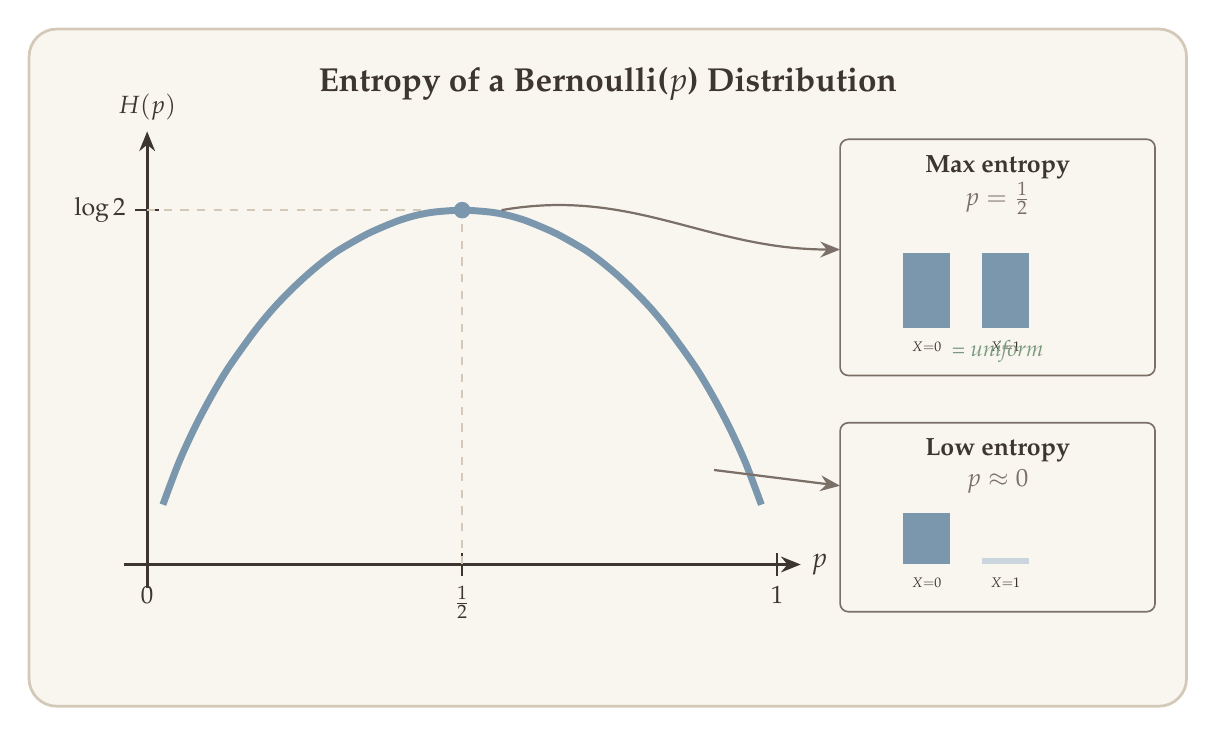
\begin{tikzpicture}[
  >={Stealth[length=2.5mm, width=2mm]},
]

% Background
\fill[cream, rounded corners=10pt] (-1.5,-1.8) rectangle (13.2,6.8);
\draw[border, rounded corners=10pt, line width=1pt] (-1.5,-1.8) rectangle (13.2,6.8);

% Title
\node[font=\large\bfseries, text=dkbrown] at (5.85,6.1)
  {Entropy of a Bernoulli($p$) Distribution};

% === Axes ===
\draw[->, line width=1pt, dkbrown] (-0.3,0) -- (8.3,0)
  node[right, font=\normalsize] {$p$};
\draw[->, line width=1pt, dkbrown] (0,-0.3) -- (0,5.5)
  node[above, font=\small] {$H(p)$};

% Tick marks on x-axis
\draw[dkbrown, line width=0.6pt] (0,-0.15) -- (0,0.15);
\draw[dkbrown, line width=0.6pt] (4,-0.15) -- (4,0.15);
\draw[dkbrown, line width=0.6pt] (8,-0.15) -- (8,0.15);
\node[font=\small, text=dkbrown, below] at (0,-0.15) {$0$};
\node[font=\small, text=dkbrown, below] at (4,-0.15) {$\tfrac{1}{2}$};
\node[font=\small, text=dkbrown, below] at (8,-0.15) {$1$};

% Tick on y-axis
\draw[dkbrown, line width=0.6pt] (-0.15,4.5) -- (0.15,4.5);
\node[font=\small, text=dkbrown, left] at (-0.15,4.5) {$\log 2$};

% Dashed line at max
\draw[border, line width=0.8pt, dashed] (0,4.5) -- (4,4.5);
\draw[border, line width=0.8pt, dashed] (4,0) -- (4,4.5);

% === Entropy curve: H(p) = -p ln p - (1-p) ln(1-p), scaled ===
% x = 8p, y = 4.5 * H(p)/log(2)
% Plot using smooth curve through computed points
\draw[stblue, line width=2.5pt, smooth, tension=0.5]
  plot coordinates {
    (0.20, 0.76)
    (0.40, 1.29)
    (0.60, 1.73)
    (0.80, 2.11)
    (1.00, 2.45)
    (1.20, 2.74)
    (1.40, 3.01)
    (1.60, 3.25)
    (1.80, 3.46)
    (2.00, 3.65)
    (2.20, 3.82)
    (2.40, 3.97)
    (2.60, 4.09)
    (2.80, 4.20)
    (3.00, 4.29)
    (3.20, 4.37)
    (3.40, 4.43)
    (3.60, 4.47)
    (3.80, 4.49)
    (4.00, 4.50)
    (4.20, 4.49)
    (4.40, 4.47)
    (4.60, 4.43)
    (4.80, 4.37)
    (5.00, 4.29)
    (5.20, 4.20)
    (5.40, 4.09)
    (5.60, 3.97)
    (5.80, 3.82)
    (6.00, 3.65)
    (6.20, 3.46)
    (6.40, 3.25)
    (6.60, 3.01)
    (6.80, 2.74)
    (7.00, 2.45)
    (7.20, 2.11)
    (7.40, 1.73)
    (7.60, 1.29)
    (7.80, 0.76)
  };

% Max point marker
\fill[stblue] (4,4.5) circle (3pt);

% === Annotations with mini bar charts ===

% --- Left annotation: p near 0 (low entropy, concentrated) ---
\draw[wmgray, line width=0.6pt, rounded corners=3pt] (8.8,-0.6) rectangle (12.8,1.8);
\node[font=\small\bfseries, text=dkbrown] at (10.8,1.45) {Low entropy};
\node[font=\small\itshape, text=wmgray] at (10.8,1.05) {$p \approx 0$};

% Mini bar chart for p~0.1: P(X=0)=0.9 tall, P(X=1)=0.1 short
\fill[stblue] (9.6,0.0) rectangle (10.2,0.65);
\fill[stblue!40] (10.6,0.0) rectangle (11.2,0.08);
\node[font=\tiny, text=dkbrown, below] at (9.9,-0.05) {$X{=}0$};
\node[font=\tiny, text=dkbrown, below] at (10.9,-0.05) {$X{=}1$};
% Arrow from curve
\draw[->, wmgray, line width=0.8pt] (7.2,1.2) -- (8.8,1.0);

% --- Middle annotation: p = 0.5 (max entropy, uniform) ---
\draw[wmgray, line width=0.6pt, rounded corners=3pt] (8.8,2.4) rectangle (12.8,5.4);
\node[font=\small\bfseries, text=dkbrown] at (10.8,5.05) {Max entropy};
\node[font=\small\itshape, text=wmgray] at (10.8,4.65) {$p = \tfrac{1}{2}$};

% Mini bar chart for p=0.5 (equal bars)
\fill[stblue] (9.6,3.0) rectangle (10.2,3.95);
\fill[stblue] (10.6,3.0) rectangle (11.2,3.95);
\node[font=\tiny, text=dkbrown, below] at (9.9,2.95) {$X{=}0$};
\node[font=\tiny, text=dkbrown, below] at (10.9,2.95) {$X{=}1$};
\node[font=\footnotesize\itshape, text=sage] at (10.8,2.7) {= uniform};
% Arrow from peak
\draw[->, wmgray, line width=0.8pt] (4.5,4.5) to[out=10,in=180] (8.8,4.0);

\end{tikzpicture}
\end{document}
